\documentclass[a4paper,twoside,11pt]{report}
\usepackage[a4paper]{geometry}
\usepackage{fullpage}
\usepackage[czech]{babel}
\usepackage[utf8]{inputenc}
\usepackage[T1]{fontenc}
\usepackage{hyperref}
\usepackage{microtype}
\usepackage{listings}
\usepackage{lmodern}
\usepackage{marginnote}
\usepackage{syntax}
\usepackage{at}
\usepackage{makeidx}
\usepackage{graphicx}
\usepackage{float}
\usepackage{caption}
\usepackage{subcaption}
\usepackage[fixlanguage]{babelbib}
\usepackage{tabularx}
\usepackage{changepage}

\selectbiblanguage{czech}

\lstloadlanguages{Haskell}

\lstdefinestyle{haskell}{
  basicstyle=\small\ttfamily,
  flexiblecolumns=false,
  basewidth=0.5em,
  language=Haskell,
  showstringspaces=false,
  keywords={ % use only real Haskell keywords
    case,class,data,default,deriving,do,else
    ,foreign,if,import,in,infix,infixl
    ,infixr,instance,let,module,newtype,of
    ,then,type,where
  },
  otherkeywords={_},
  texcl=true,
}

% code chunks in literate haskell
\lstnewenvironment{code}{\lstset{style=haskell}}{}
% code chunks which should NOT be processed by literate haskell
\lstnewenvironment{code*}{\lstset{style=haskell}}{}

\lstdefinestyle{krunimir}{
  basicstyle=\small\ttfamily,
  flexiblecolumns=false,
  basewidth=0.5em,
  keywords={
    forward,left,right,color,pen,split,if,repeat,define
  },
}

\DisableLigatures[>,<]{encoding = T1,family=tt*} %
\setlength{\grammarparsep}{5pt plus 1pt minus 1pt} 
\setlength{\grammarindent}{12em}

\renewcommand*{\marginfont}{\scriptsize}

\newatcommand t[1]{\texttt{#1}}

\makeindex
\newatcommand idx[1]{\index{#1@\texttt{#1}}}
\newatcommand Idx[1]{\index{#1@\texttt{#1}|textbf}}

\hypersetup{
  unicode=true,          % non-Latin characters in Acrobat’s bookmarks
  pdftitle={TITULEK !!!!!},    % title
  pdfauthor={Jan Špaček},     % author
  hidelinks,
  % hyperindex should be true by default, hyperref shows warning 
  % "Option `hyperindex' has already been used,"
  % hyperindex=true,
  linktoc=all,
}

\begin{document}
%%% The halftitle

\setcounter{page}{-99}

\begin{titlepage}
\begin{center}

\textsc{\LARGE Středoškolská odborná činnost}\\[4cm]

\textsc{\Huge Líně, čistě,\\ funkcionálně}\\[0.5cm]

\textit{\LARGE Užití funkcionálního programovacího jazyka Haskell k řešení
úloh Ústředních kol ČR Soutěže v programování}\\[2.5cm]

\textsc{\huge Jan Špaček}\\[11.5cm]

\textit{\LARGE Ostrava 2013}

\end{center}
\end{titlepage}

% hides the page number
\thispagestyle{empty}
\cleardoublepage

%%% The title

\begin{center}

\textsc{\LARGE Středoškolská odborná činnost}\\[0.6cm]
\textsc{\large Obor SOČ: 18 Informatika}\\[2cm]

\textsc{\Huge Líně, čistě,\\ funkcionálně}\\[0.5cm]

\textit{\LARGE Užití funkcionálního programovacího jazyka Haskell k řešení
úloh Ústředních kol ČR Soutěže v programování}\\[2cm]

\textsc{\huge Lazily, purely, functionally}\\[0.3cm]

\textit{\Large Using the functional programming language Haskell to solve
tasks from the finals of the Czech Programming Contest}\\[5cm]

\begin{tabularx}{12cm}{
  >{\Large\scshape}p{3cm} 
  >{\LARGE\scshape}X 
}
Autor:    & Jan Špaček \\[0.5cm]
% aww, how dirty! :)
Škola:    & Wichterlovo gymnázium \\[0.15cm]
          & Čs.~exilu 669 \\[0.2cm]
          & Ostrava-Poruba \\
\end{tabularx}
\\[3cm]

\textit{\LARGE Ostrava 2013}

\end{center}

\setcounter{page}{1}
\thispagestyle{empty}

\newpage

%%% QR code to github.com

~\\[3cm]
\begin{center}

\includegraphics[width=5cm]{img/github-head-qr}
\end{center}

%%% The declaration

~\\[7cm]
\section*{Prohlášení}

Prohlašuji, že jsem svou práci vypracoval samostatně, použil jsem pouze
podklady (literaturu, SW atd.) uvedené v přiloženém seznamu a postup při
zpracování a dalším nakládání s prací je v souladu se zákonem č. 121/2000 Sb.,
o právu autorském, o právech souvisejících s právem autorským a o změně
některých zákonů (autorský zákon) v platném znění.\\[0.7cm]

V \makebox[3cm]{\dotfill} dne \makebox[4cm]{\dotfill}
podpis: \makebox[6cm]{\dotfill}

\newpage

% The "Thanks" page
~

\newpage

\tableofcontents
\chapter{Krunimír: želví grafika}

\begin{quotation}

Želvák Krunimír je velký myslitel. Zjistil, ze když si za krunýř přiváže trochu
křídy, kreslí za sebou při svém plazení cestičku. I pojal plán nakreslit svoji
podobiznu, samozřejmě včetně přesných detailů krunýře. Hned se dal pln nadšení
do díla a práce mu šla pěkně od ... tlapy.

\uv{Co to děláš, dědečku,} zeptal se jednou Krunimíra jeho vnuk Krunoslav.
\uv{Krešlím tady švou poďobižnu,} odpověděl Krunimír. \uv{Žačal jsem š ní, když
tvůj tatík ještě nebyl na švětě, a ještě nemám ani krunýř,} dodal smutně. \uv{To
už ji aši dokrešlit neštihnu...}  Vnuk Krunoslav, znalec moderní techniky, mu
však poradil: \uv{Tak si nech napsat program, který ji nakreslí za Tebe.}
Protože se ale s tlapami a zobákem moc dobře neprogramuje, najali si želváci
vás.

\end{quotation}

Takto začíná zadání finální úlohy Soutěže v programování z roku 2010. Popisuje
jednoduchý procedurální jazyk na generování želví grafiky, inspirovaný jazykem
Logo, a úkolem je vytvořit interpret tohoto jazyka, jehož vstupem je text
programu a výstupem vykreslený obrázek.

\marginnote{Hodil by se nějaký popsaný obrázek s výsledkem Krunimírovy práce,
třeba některý ze stromů.}

\begin{figure}
  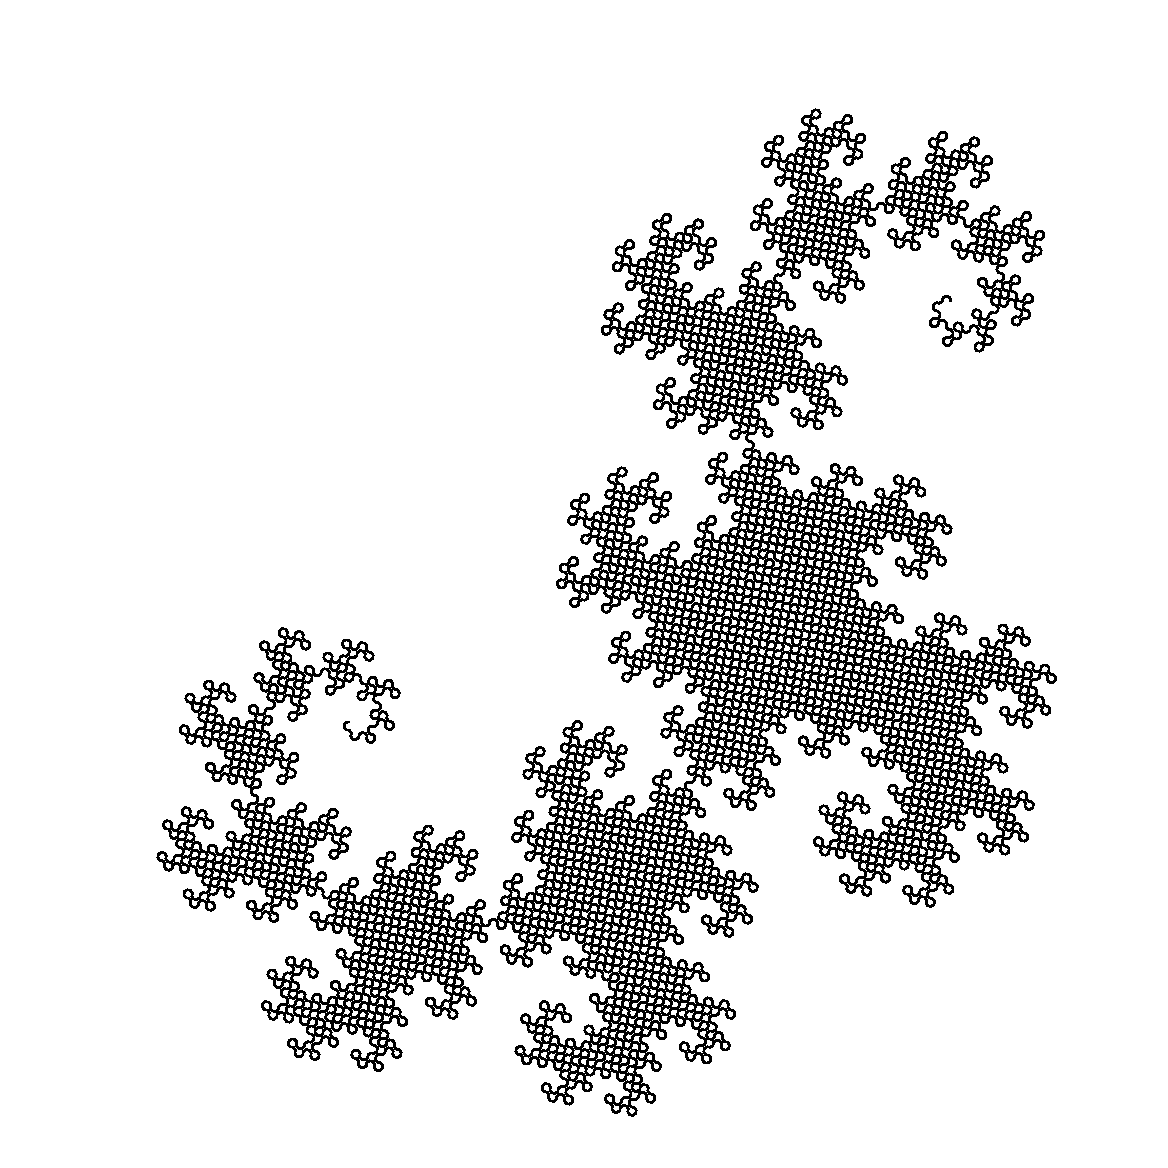
\includegraphics[width=0.9\textwidth]{krunimir/examples/dragon}
  \caption{Příklad obrázku vykresleného pomocí Krunimírova jazyka (Dračí křivka)}
  \label{fig:krunimir-dragon}
\end{figure}

\section{Popis jazyka}

Uživatel má k dispozici několik primitivních kreslících funkcí:

\begin{description}
\item[@t{forward(d)}] Želva se posune vpřed o @t{d} jednotek (pixelů).
Pokud je tloušťka pera kladná, zanechá za sebou čáru vedoucí z původní pozice do
nové. Takovýto pohyb se považuje za jeden \emph{tah}.
\item[@t{right(a)}, @t{left(a)}] Želva se otočí doprava, resp. doleva o
@t{a} stupňů.
\item[@t{pen(s)}] Nastaví tloušťku pera na @t{s}
\item[@t{color(r, g, b)}] Nastaví barvu pera, @t{r}, @t{g} a
@t{b} jsou jednotlivé složky modelu RGB v rozsahu 0 až 255.
\end{description}

Jazyk dále umožňuje použít jednoduchou podmínku a cyklus:

\begin{description}
\item[@t{if(x) \{ ... \}}] Vykoná příkazy v těle podmínky právě když je
@t{x} kladné.
\item[@t{repeat(x) \{ ... \}}] Vykoná příkazy @t{x}-krát, je-li
@t{x} kladné.
\end{description}

Uživatel může definovat vlastní procedury a volat je:

\begin{description}

\item[@t{define 
  \textit{procedura}(\textit{p1},\textit{p2},...)
  \{ ... \}
}]
  Definuje proceduru \textit{procedura}, která má libovolný počet parametrů
  (\textit{p1}, \textit{p2}, ...). Tyto parametry mohou být v těle procedury
  použity ve výrazech a nabývají hodnoty předané v místě volání.

\item[@t{\textit{procedura}(\textit{arg1},\textit{arg2},...)}]
  Zavolá proceduru \textit{procedura} s argumenty (\textit{arg1}, \textit{arg2},
  ...). Procedura musí být definována \textit{před} svým voláním a může být
  rekurzivní.

\end{description}

Poslední a nejzajímavější struktura je rozdvojení:

\begin{description}
\item[@t{split \{ ... \}}] Vytvoří klon aktuální želvy, která vykoná
příkazy v těle struktury @t{split}, přičemž původní želva pokračuje ve vykonávání
dalších příkazů. Všechny želvy se pohybují paralelně, vždy všechny provedou
jeden \emph{krok}, poté druhý atd.
\end{description}

Jako argumenty při volání procedur lze používat výrazy vytvořené z celočíselných
literálů, parametrů aktuální procedury, binárních operátorů @t{+}, @t{-},
@t{*} a @t{/} (celočíselné dělení) a negace pomocí operátoru
@t{-}. Ve výrazech je možno používat závorky @t{(} a @t{)},
priorita a asociativita operátorů je jako v matematice.

\subsection{Příklady}

Výstupy těchto příkladů jsou na obrázku \ref{fig:krunimir-examples}.

\subsubsection{Čtverec (\ref{fig:krunimir-square1})}

Jednoduchý kód, který vykreslí čtverec. 
\lstinputlisting[style=krunimir]{krunimir/examples/square1.txt}

\subsubsection{Mřížka čtverců (\ref{fig:krunimir-squares})}

V této ukázce využijeme procedury, abychom kód rozdělili na menší a přehlednější
části.
\lstinputlisting[style=krunimir]{krunimir/examples/squares.txt}

\subsubsection{Binární strom (\ref{fig:krunimir-bintree})}

Při vykreslování stromů prokáže svoji užitečnost příkaz @t{split}.
\lstinputlisting[style=krunimir]{krunimir/examples/bintree.txt}

% příklady a jejich výsledky by opravdu neměly utéct někam pryč, proto H
\begin{figure}[H]
  \centering

  \begin{subfigure}{0.3\textwidth}
    \centering
    
\includegraphics[width=\textwidth]{krunimir/examples/square1}
    \caption{Čtverec}\label{fig:krunimir-square1}
  \end{subfigure}
  ~
  \begin{subfigure}{0.3\textwidth}
    \centering
    
\includegraphics[width=\textwidth]{krunimir/examples/squares}
    \caption{Mřížka čtverců}\label{fig:krunimir-squares}
  \end{subfigure}
  ~
  \begin{subfigure}{0.3\textwidth}
    \centering
    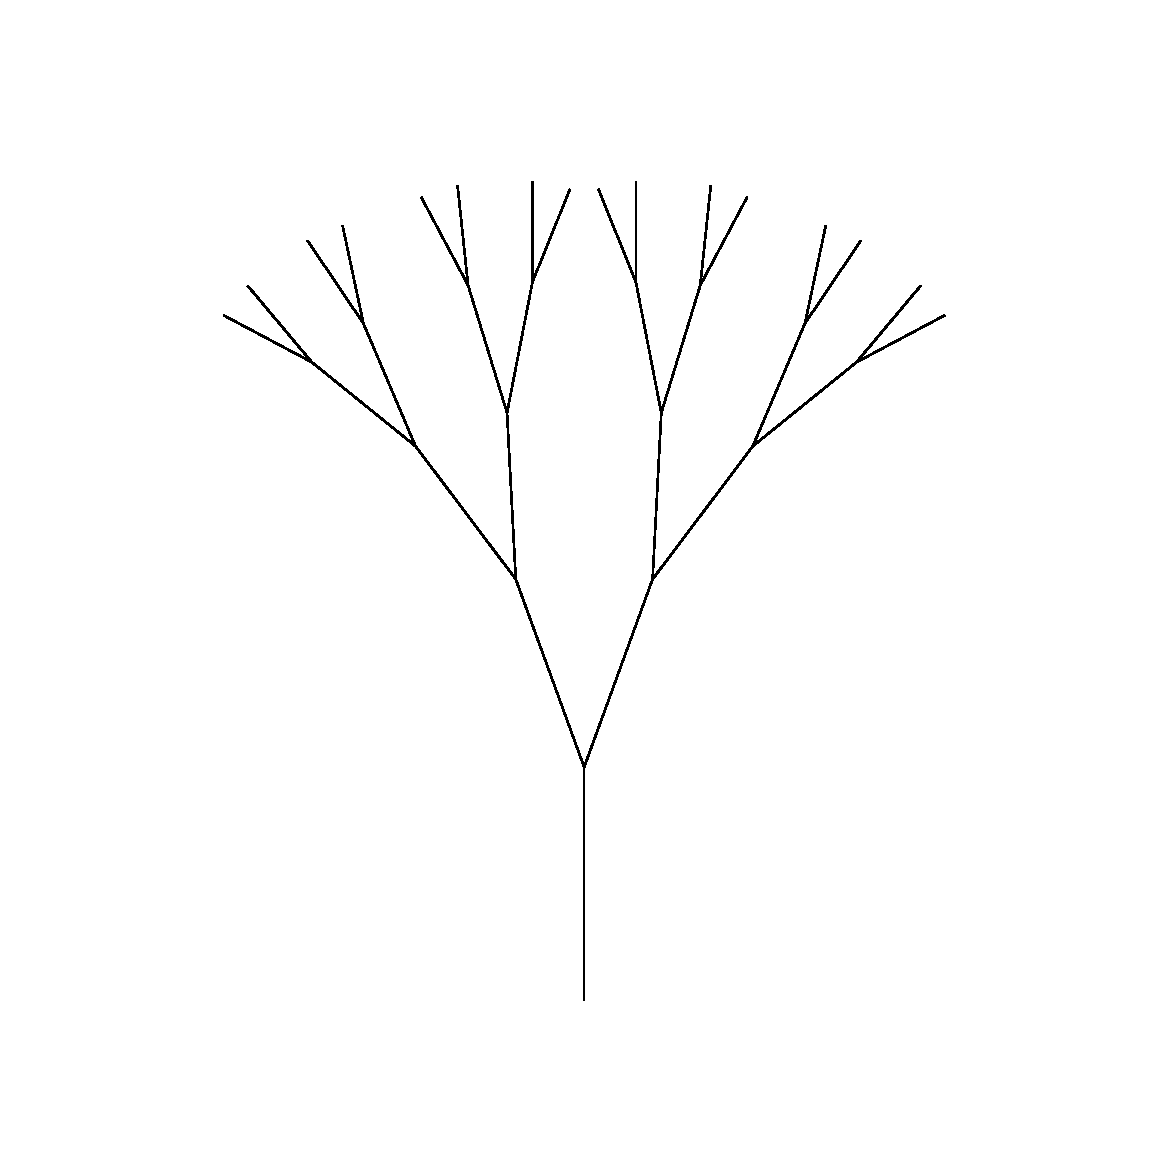
\includegraphics[width=\textwidth]{krunimir/examples/bintree}
    \caption{Binární strom}\label{fig:krunimir-bintree}
  \end{subfigure}

  \caption{Výsledné obrázky z příkladů}
  \label{fig:krunimir-examples}
\end{figure}

\section{Analýza}

Problém si můžeme rozdělit na tři části:

\begin{enumerate}

\item \emph{Syntaktická analýza} (\uv{parsování}) zpracuje vstupní řetězec na
  \emph{abstraktní syntaktický strom}, který zachycuje strukturu programu ve
  formě, která je jednoduše zpracovatelná v dalších fázích.

\item Následuje \emph{vyhodnocení}, kdy ze syntaktického stromu vypočteme
  výslednou stopu (ve vektorové podobě jako seznam úseček).

\item Poslední částí je \emph{vykreslení}, které vykreslí vyhodnocenou stopu do
  obrázku. Budeme exportovat do rastrových obrázků formátu PNG a vektorových
  formátu SVG.

\end{enumerate}

Pomocí tohoto jednoduchého rozdělení můžeme naše řešení rozvrhnout do sedmi
modulů:

\begin{description}

\item @t{Krunimir.Main} exportuje @t{main}, která slouží jako rozhraní s
uživatelem. \footnote{Podobně jako funkce @t{main()} v jazyku C}
  @idx{Krunimir.Main}
  @idx{Krunimir.Main.main}

\item @t{Krunimir.Parser} exportuje funkci @t{parse}, která z textového
zápisu programu vytvoří syntaktický strom (nebo syntaktickou chybu).
  @idx{Krunimir.Parser}
  @idx{Krunimir.Parser.parse}

\item @t{Krunimir.Ast} definuje datové typy, které reprezentují syntaktický
strom.
  @idx{Krunimir.Ast}

\item @t{Krunimir.Evaluator} poskytuje funkci @t{eval}, která ze
syntaktického stromu vypočte výslednou stopu.
  @idx{Krunimir.Evaluator}
  @idx{Krunimir.Evaluator.eval}

\item @t{Krunimir.Trace} definuje datové typy a funkce spojené se stopou želvy.
  @idx{Krunimir.Trace}

\item @t{Krunimir.PngRenderer} exportuje funkci @t{renderPng}, která vykreslí
  stopu jako PNG obrázek.
  @idx{Krunimir.PngRenderer}
  @idx{Krunimir.PngRenderer.renderPng}

\item @t{Krunimir.SvgRenderer} poskytuje funkci @t{renderSvg}, jenž uloží stopu
  ve vektorovém formátu SVG.
  @idx{Krunimir.SvgRenderer}
  @idx{Krunimir.SvgRenderer.renderSvg}

\end{description}

\input{krunimir/Krunimir/Main.lhs}
\input{krunimir/Krunimir/Ast.lhs}
\input{krunimir/Krunimir/Parser.lhs}
\input{krunimir/Krunimir/Trace.lhs}
\input{krunimir/Krunimir/Evaluator.lhs}
\input{krunimir/Krunimir/PngRenderer.lhs}
\input{krunimir/Krunimir/SvgRenderer.lhs}

\printindex

\bibliographystyle{babplain}
\bibliography{bibliography}

\end{document}
